%!TEX root = ../dissertation.tex

\chapter{Data authentication in Galileo}

So far we've described the classic radio satellite navigation problem and
solution. This generally accepted model works well but provides no security
guarantees. In particular, it doesn't prevent malicious users to forge ad-hoc
signals and impersonate a satellite, or even a whole GNSS.

In this chapter we'll describe the general data authentication problem for open
signals in GNSS environments, the threat model and the possible attacks. We will
then move on to describe TESLA, a data authentication protocol suited for
streaming, lossy channels that the Galileo program chose to implement in order
to secure the navigation message. We'll also describe the proposed
implementation of TESLA in the current Galileo subframe structure.

\section{TESLA}
Certain characteristics of the Galileo signal make the problem of authenticating
the data very peculiar. Among others:
\begin{itemize}
  \item communication is unidirectional, from satellite to receiver(s)
  \item receivers can connect at any point in time
  \item the channel is lossy and doesn't guarantee data delivery
  \item communication happen on a very low-speed channel
\end{itemize}
The first three traits make it easier to associate the Galileo signal to a
multicast streaming communication. For this kind of communication, two schemes
have been proposed in \cite{perrig}. One of them, TESLA, offers authentication
of the sender with a minimal overhead, strong loss resistance and high
scalability, at the price of slightly delayed authentication. The second of
them, EMSS, adds non-repudiation on top of those features. The Galileo
commission chose to implement TESLA, and therefore we'd now put our focus on it.

\par

As an overview, TESLA builds on top of classic asymmetric authentication schemes
and MAC for data authentication. What TESLA does is to authenticate the data it
sends and to disclose the key that authenticated that data in a later packet.
Moreover, keys are connected with each other by using a key generation function
that takes a previous key as input. To account for different reception speeds,
TESLA supports using multiple chains, each with a different validity time for a
single key.

In our overview of the algorithm, we'll first look at how a single key chain
works, and then extend the concept to multiple chains.

\par

We start from a stream of messages $M_j$, each one sent after the other and
received in the same sequence. For each of these messages, TESLA computes a MAC
using a key $K_i$ and attaches it to the message. Moreover, TESLA attaches to
the same message the key it used to authenticate a previous message
$M_{j-\delta}$, where $\delta$ is a parameter called \textit{disclosure lag},
chosen so that it's guaranteed that every receiver received $M_{j-\delta}$ by
the time $M_j$ is sent out. This is referred as the \textit{security condition}
of the TESLA protocol, and it means that there's no chance for an attacker to
read $M_j$, tamper $M_{j-\delta}$ and have the latter accepted by a receiver.

Since keys are disclosed in clear, TESLA provides a way to verify that the key
is authentic by using other keys in the chain, plus a bootstrap mechanism. The
sender start by generating a random key $K_l$ that remains secret and that's
never used to sign any message. After this, the sender computes a chain of keys
by successively applying a one-way function $F$ to the keys in the chain:

\[
  K_i = F(K_{i+1})
\]

After $l$ steps, the chain is complete and the last application of $F$ yields
what's called a \textit{root key}:

\[
  K_0 = F^l(K_l)
\]

At this point the keys are broadcasted in reverse order than they're computed,
i.e. $K_0$ is sent before $K_1$, etc. This makes so that it's computationally
infeasible for an attacker to calculate $K_{i+1}$ given $K_i$ since $F$ is a
cryptographically secure one-way function. At the same time, once a receiver
receives $K_{i+1}$, it's easy for it to verify that the key $K_i$ is authentic,
as it needs to only apply $F$ to $K_{i+1}$ once and verify that the result is
$K_i$. The only requirement is that the root key is signed using a normal
asymmetric scheme during a bootstrap phase, so that receivers can verify that
the chain has been generated by the legitimate sender.

Another important aspect of TESLA is the use of the same key across several
messaeges. In fact, the validity of a key is not tied to a number of messages
but rather to an amount of time. This way the underlying streaming protocol can
have a variable streaming rate without increasing the overhead on the receiver's
side.

To give support to different types of receivers with different network access
speed, TESLA suggests the implementation of multiple simultaneous chains with
different disclosure periods $\delta$.

One important precondition that needs to be satisfied for the security condition
to hold is that sender and receivers have clocks that are roughly in sync within
a disclosure period (otherwise the security condition cannot be practically
verified).

\section{Galileo OSNMA}
In 2016, a specification for a data authentication protocol in Galileo has been
released under the name of OSNMA \cite{osnma}. This specification builds on top
of the TESLA algorithm just described with a few notable exceptions. We'll give
here an introduction to this protocol to contextualize the analysis that
follows.

\par

The OSNMA specification describes two distinct sets of information that are sent
along together but at different rates: the HKROOT and the MACK sections. The
HKROOT contains a set of headers needed to correctly interpret the
authentication data, the root key of the chain in force and its digital
signature. The MACK section contains a configurable number of MAC which
authenticate different groups of fields contained in the navigation message, and
the key with which the MAC are generated.

These two pieces of information are transmitted together at a rate of 40 bits
per page (2s) in the field called "Reserved 1" in the Galileo ICD
\cite{galileoicd}. The HKROOT section occupies 8 of those bits, while the
remaining 32 are allocated for the MACK section.

\begin{figure}[h!]
  \begin{center}
    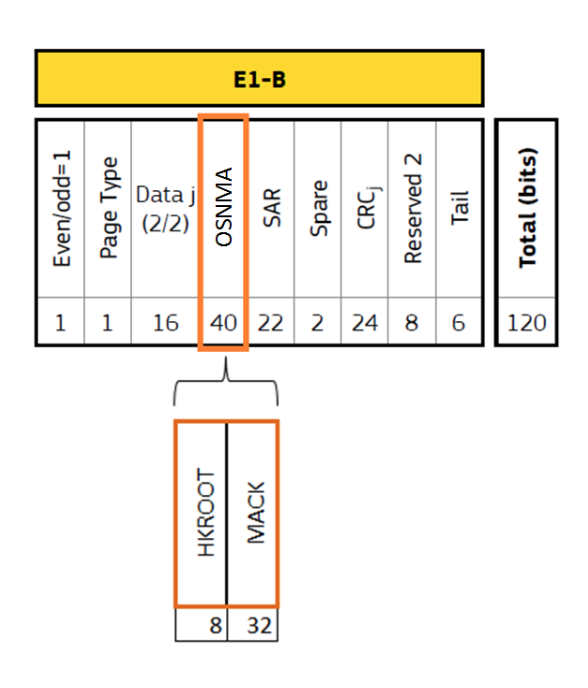
\includegraphics[width=0.5\textwidth]{figures/osnma_fields.png}
  \end{center}
  \caption{OSNMA message structure in Galileo E1B I/NAV frame}
  \label{fig:osnma_fields}
\end{figure}

In total, a HKROOT section has a variable length and it's transmitted in blocks
of 104 bits - one block per subframe. The MACK section instead has a fixed
length of 480 bits and can contain a variable number of MACs and keys (up to 480
bits; the remaining bits are padded).

The HKROOT can also be thought as composed of two sections: the header and the
DSM-KROOT. The header contains information about the overall NMA status and
about the DSM transmitted in the section. The first header is composed of three
fields: the operational status of NMA, the status of the DSM and the ID of the
chain in force. The second header contains the ID of the DSM, which identifies
also if the transmitted information is related to a root key being
authenticated, or if it's a message related to a key revocation. Also, an
indication of the current block being received is sent in this header. The
DSM-KROOT instead contains a set of parameters like the total number of blocks,
the hash function to be used and the key size, together with the DSM and the
associated key. The DSM-KROOT can be optionally be swapped with the DSM-PKR
section for key revocation.

\begin{figure}[h!]
  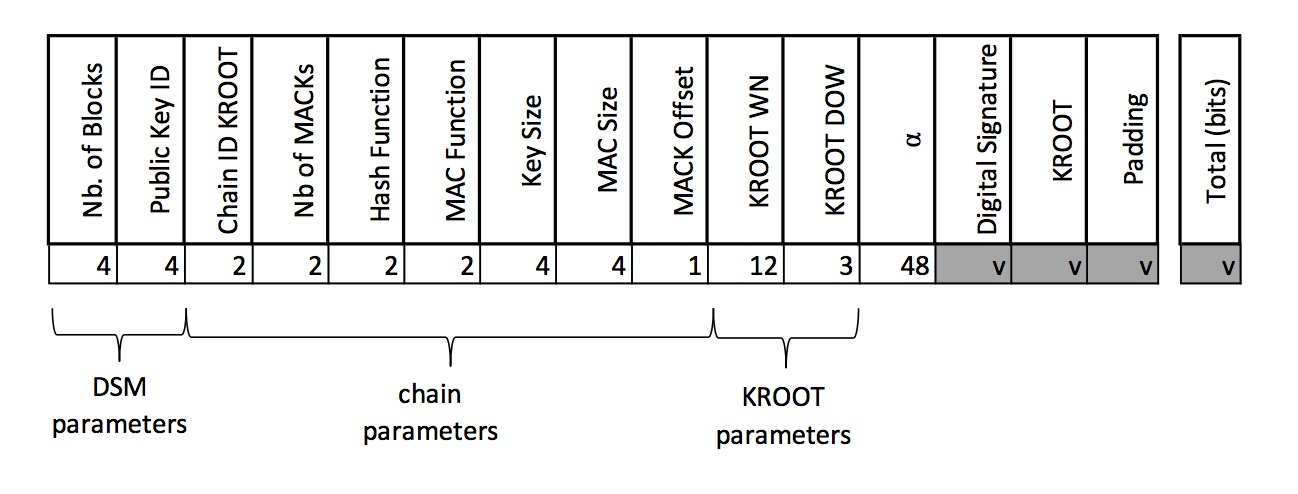
\includegraphics[width=\linewidth]{figures/dsm_kroot.png}
  \caption{Fields in DSM-KROOT section. "v" in the bit size stands for "variable"}
  \label{fig:dsm_kroot}
\end{figure}

The MACK section instead contains the authentication codes for the data
transmitted in the navigation message. This data is authenticated with different
MAC, therefore the MACK message also contains information on what data is
included in the message from which the MAC has been generated, in the form of a
4 bit field called ADKD (Authentication Data \& Key Delay). Together with this,
the PRN of the satellite being authenticated and an Issue of Data field
indicating if the data transmitted is new are sent.

After the MACs, the key that generated them follows, the size of which is
specified in the DSM.

\begin{figure}[h!]
  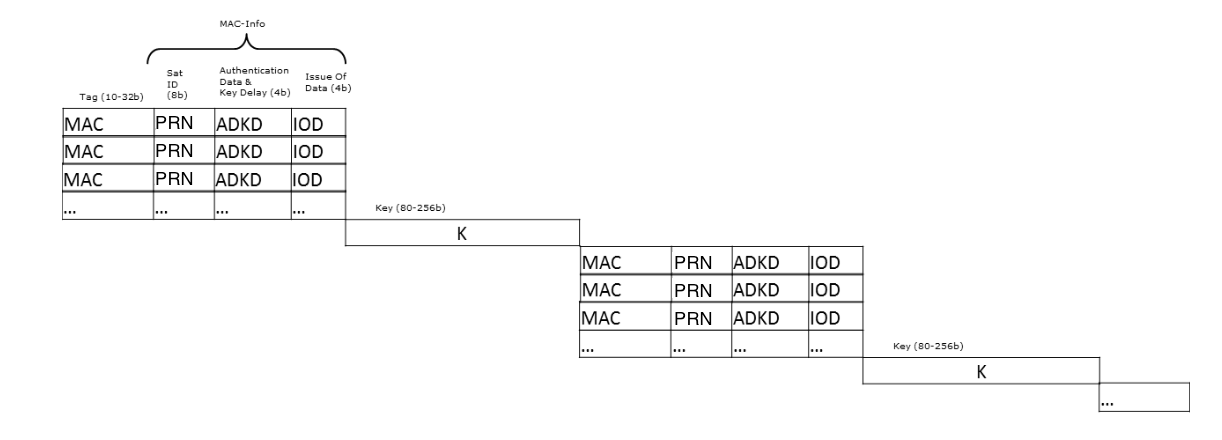
\includegraphics[width=\linewidth]{figures/mack.png}
  \caption{MACK section structure}
  \label{fig:dsm_kroot}
\end{figure}

The pieces of information included in OSNMA are to be used by the receiver as
follows:
\begin{itemize}
\item the receiver must first receive and decode in full the root key $K_R$
transmitted in the DSM
\item the receiver computes the DSM for the root key as follows
\begin{align*}
& M = (\text{NMA\_Header} \Vert \text{CIDKR} \Vert \text{NMACK} \Vert \text{HF}
\Vert \text{MF} \Vert \text{KS} \Vert \text{MS} \Vert \text{MO} \Vert \\
& \text{KROOT WN} \Vert \text{KROOT DOW} \Vert \alpha \Vert K_R) \\
\\
& S = signature(M, K_{pub})
\end{align*}

where for $signature()$ ECDSA is proposed in \cite{osnma} with several supported
signature lengths, the actual value of it is univocally identified by the
\textit{Public Key ID} transmitted in the DSM header. $K_{pub}$ is the public
key identified by mentioned ID and built in into the receiver. All the other
parameters are defined in \cite{osnma}.

If the computed signature matches the received DSM, then the received KROOT is
to be considered valid
\item once the root key has been verified, the receiver can start to read a MACK
section, and then decode the MACs and the key $K_j$ associated to them.
Depending on how the protocol is configured, the receiver might have to decode
the next subframe to get the key that generated the MACs in its possession.
\item the receiver identifies the distance $d$ between the root key $K_R$ and
the key sent in the MACK section $K_j$
\item the receiver verifies the key sent in the MACK section against the root
key already verified by applying $d$ times the key generating function $F$ on
$K_j$:
\[
K'_R = F^m(K_j)
\]
\item the receiver verifies that $K'_R = K_R$. If the equality holds true, then
the data received is legitimated and the receiver can proceed in verifying the
actual data in the navigation message against the MACs already received.
\item the navigation data is verified by building a message in the format
\[
m = (\text{PRN\_N} \Vert \text{PRN\_A} \Vert GST_{SF} \Vert \text{CTR} \Vert
\text{NMA\_Status\_Header} \Vert \text{navdata})
\]
where $\text{PRN\_N}$ is the PRN of the satellite being authenticated,
$\text{PRN\_A}$ is the PRN of the satellite sending the authentication data,
$GST_{SF}$ is the Galileo system time of the start of the subframe in which the
MAC is contained, $CTR$ is the position of the MAC in the MACK section,
$\text{NMA\_Status\_Header}$ is the NAM status field in the NMA header, and
$\text{navdata}$ is fetched looking into the ADKD field of the MAC-Info section
of the MAC and combining the data field according to \cite{osnma}. The message
thus constructed is then verifying by applying to it the hash function specified
by the protocol together with the key $K_j$. If the resulting hash, truncated
accordingly to the MAC length specified in the protocol configuration, matches
the MAC in possession of the receiver, then the data is considered authenticated
and valid.
\end{itemize}

\par

One important aspect of OSNMA is the generation of the key chain. According to
the protocol, the ground segments generates one chain that's valid for all
satellites. This means that when two subsequent keys $K_i$ and $K_j$ are
received from a same satellite, they're not at one step distance (i.e. $K_i =
F(K_j)$ doesn't hold) but in between them there are other 35 keys, one for each
satellite (where the total number of satellites is nominally 36 but should be
configurable according to the specification).
